% Gestão e feedback v0.8 - apresentação UFG, 23/11/2026.
% 34 slides | 37 min + 3 min de reserva. Compilar nesta pasta.
\documentclass[aspectratio=169,t,xcolor=table]{beamer}
\usepackage[utf8]{inputenc}
\usepackage[brazil]{babel}
\usepackage{booktabs,tabularx,listings,qrcode}
\usetheme{Ufg}
\definecolor{Navy}{HTML}{12334B}
\definecolor{Muted}{HTML}{526574}
\definecolor{PaleBlue}{HTML}{EAF3F9}
\setPrimaryColor{UFGBlue}
\setLogos{lib/logos/INF-compact-white.png}{lib/logos/INF-compact-white.png}
\setbeamertemplate{navigation symbols}{}
\setbeameroption{hide notes}
\setbeamerfont{frametitle}{size=\Large,series=\bfseries}
\setbeamercolor{frametitle}{fg=Navy}
\newcolumntype{L}[1]{>{\raggedright\arraybackslash}p{#1}}
\newcolumntype{Y}{>{\raggedright\arraybackslash}X}
\renewcommand{\arraystretch}{1.16}
\setlength{\tabcolsep}{5pt}
\newcommand{\head}[1]{\textcolor{UFGBlue}{\textbf{#1}}}
\newcommand{\kicker}[1]{{\footnotesize\bfseries\color{UFGBlue}#1\par}\vspace{.18cm}}
\newcommand{\num}[1]{{\fontsize{31}{34}\selectfont\bfseries\color{UFGBlue}#1}}
\newcommand{\aside}[1]{{\fontsize{8}{10}\selectfont\color{Muted}#1\par}}
\title[Gestão e feedback]{Requisitos de um sistema de gestão e feedback}
\subtitle{Levantamento e especificação de requisitos}
\author[Equipe PulsarRH]{Brenner Rodrigues Sardinha \and Danilo Sucupira Galvão \and Enzo de Oliveira Machado \and Heitor Barbosa Souza \and Luiz Augusto Vaz}
\institute{Instituto de Informática -- Universidade Federal de Goiás}
\date{Novembro de 2026}
\hypersetup{pdftitle={Requisitos de um sistema de gestão e feedback},pdfauthor={Equipe PulsarRH},pdfsubject={Domínios de Software - UFG - 2026/2}}

\usepackage{pulsarrh-modern}

\newcommand{\sumitem}[3]{%
  {\color{UFGBlue}\bfseries #1\enspace\textcolor{Navy}{#2}\par}%
  \vspace{.07cm}{\fontsize{9}{12}\selectfont #3\par}\vspace{.30cm}}
\newcommand{\reqitem}[3]{%
  {\color{UFGBlue}\bfseries #1\enspace\textcolor{Navy}{#2}\par}%
  \vspace{.14cm}#3\par\vspace{.42cm}}



\begin{document}
\section{Contexto}
\subsection{Feedback e objetivo do trabalho}
% Slide 01 | 0.5 min
\begingroup\sectionopeningtrue
\setBGColor{white}
\setLayout{horizontal}
\begin{frame}{}

\begin{columns}[c,onlytextwidth]
\column{.49\textwidth}
{\fontsize{24}{28}\selectfont\bfseries\color{Navy}Requisitos de um\par sistema de gestão\par e feedback\par}
\vspace{.25cm}
{\normalsize\bfseries Levantamento e especificação\par}
\vspace{.25cm}
{\small Domínios de Software | UFG\par Novembro de 2026\par}
\column{.49\textwidth}

\includegraphics[width=\linewidth]{assets/feedback-equipe.png}
\end{columns}
\vspace{.22cm}
{\fontsize{7}{9}\selectfont\color{Muted}
Brenner Rodrigues Sardinha \textbullet\ Danilo Sucupira Galvão\par
Enzo de Oliveira Machado \textbullet\ Heitor Barbosa Souza \textbullet\ Luiz Augusto Vaz\par}

\note{Tempo: 0.5 minuto(s). Apresentar a proposta e a equipe: Brenner Rodrigues Sardinha, Danilo Sucupira Galvão, Enzo de Oliveira Machado, Heitor Barbosa Souza e Luiz Augusto Vaz. Explicar o recorte: trabalho de levantamento e especificação, com protótipo. Não é uma aplicação implementada. A ilustração é conceitual, gerada por IA. Fonte: README.md; ilustração conceitual gerada com imagegen.}
\end{frame}
\endgroup

% Slide 02 | 1.25 min
\setBGColor{white}
\setLayout{horizontal}
\begin{frame}{O que torna um feedback útil?}

\begin{columns}[T,onlytextwidth]
\column{.35\textwidth}
\kicker{UMA FALA VAGA}
{\Large\bfseries\color{Navy}``Você precisa\par melhorar.''\par}
\vspace{.35cm}
Qual situação?\par\vspace{.12cm}
O que precisa mudar?\par\vspace{.12cm}
Como perceber a evolução?
\column{.60\textwidth}
\kicker{UMA CONVERSA QUE PERMITE AGIR}
{\large\color{Navy}``Na reunião de ontem, você interrompeu a apresentação duas vezes. O time perdeu a sequência da discussão. Na próxima, vamos anotar as dúvidas e retomá-las ao final.''\par}
\vspace{.3cm}
\textbf{A pessoa entende o que aconteceu, o efeito do comportamento e o que pode fazer na próxima situação.}
\end{columns}

\note{Tempo: 1.25 minuto(s). Tempo de abertura conceitual: contrastar uma avaliação vaga com uma devolutiva concreta. O exemplo de reunião é fictício. Um feedback útil descreve comportamentos observáveis, explicita seus efeitos e permite reconhecer o que manter ou combinar o que melhorar. A estrutura dos registros será apresentada depois, no RF21. A base conceitual vem das anotações e da síntese das entrevistas, seções 2.1 e 2.4; não tratar o exemplo como ocorrência relatada pela professora.}
\end{frame}

% Slide 03 | 0.75 min
\setBGColor{white}
\setLayout{horizontal}
\begin{frame}{Sumário}

\begin{columns}[T,onlytextwidth]
\column{.48\textwidth}
\sumitem{1}{Contexto}{1.1 Feedback e objetivo do trabalho}
\sumitem{2}{Organização do trabalho}{2.1 Divisão das tarefas e Kanban\\2.2 Branches, revisão e repositório}
\sumitem{3}{Levantamento de requisitos}{3.1 Entrevista com a professora\\3.2 Pesquisa geral\\3.3 Sistemas análogos}
\column{.48\textwidth}
\sumitem{4}{Principais requisitos}{4.1 Registro e classificação\\4.2 Avaliação e desenvolvimento\\4.3 Preservação e qualidade}
\sumitem{5}{Resultados e demonstrações}{5.1 Documentos e rastreabilidade\\5.2 Protótipo e percursos}
\sumitem{6}{Encerramento}{6.1 Síntese das entregas}
\end{columns}

\note{Tempo: 0.75 minuto(s). Apresentar o objetivo acadêmico, a metodologia e o percurso da fala. A organização do trabalho entra antes do levantamento; a demonstração dos arquivos vem depois dos requisitos. A apresentação permanece sem uma seção de modelagem. Fonte: README.md e processo de requisitos.}
\end{frame}

\section{Organização do trabalho}
% Slide 04 | 0.5 min
\begingroup\sectionopeningtrue
\setBGColor{white}
\setLayout{horizontal}
\begin{frame}{Organização do trabalho}
\begin{columns}[T,onlytextwidth]
\column{.30\textwidth}\num{01}\par\textbf{Equipe e tarefas}\par\vspace{.2cm}Responsabilidades e principais contribuições.
\column{.30\textwidth}\num{02}\par\textbf{Acompanhamento}\par\vspace{.2cm}Kanban e evolução das tarefas.
\column{.30\textwidth}\num{03}\par\textbf{Colaboração}\par\vspace{.2cm}Branches, revisão e organização dos arquivos.
\end{columns}

\note{Tempo: 0.5 minuto(s). Anunciar a organização do trabalho: apresentar a divisão de responsabilidades, o quadro de tarefas e o fluxo de revisão e integração dos documentos. Nos próximos slides, demonstrar os registros reais do GitHub.}
\end{frame}
\endgroup

\subsection{Divisão das tarefas e Kanban}
% Slide 05 | 1 min
\setBGColor{white}
\setLayout{horizontal}
\begin{frame}{Divisão das tarefas na equipe}

\small
\begin{tabularx}{\textwidth}{@{}L{.17\textwidth}YL{.25\textwidth}@{}}
\toprule\head{Integrante} & \head{Principais contribuições} & \head{Registros}\\\midrule
\textbf{Brenner} & Pesquisa, entrevistas e protótipo. & CU-01; \#3, \#22, \ldots\\[.1cm]
\textbf{Danilo} & Rastreabilidade e consistência dos artefatos. & CU-05; \#24, \#46, \ldots\\[.1cm]
\textbf{Enzo} & Sistema análogo e análise de resultados. & CU-04; \#9, \#41, \ldots\\[.1cm]
\textbf{Heitor} & Processo, Kanban e síntese das entrevistas. & CU-03; \#2, \#6, \ldots\\[.1cm]
\textbf{Luiz Augusto} & Visão, especificações e dicionário de dados. & CU-02; \#12, \#23, \ldots\\\bottomrule
\end{tabularx}\par
\vspace{.2cm}

\note{Tempo: 1 minuto(s). Explicar a distribuição com tarefas concretas, sem sugerir exclusividade: vários artefatos receberam colaboração e revisão de outras pessoas. Cada integrante produziu um caso de uso completo, como registra o índice de casos de uso. As demais contribuições foram conferidas nas issues e PRs do GitHub em 23/11/2026. Fontes: docs/casos-de-uso/README.md; issues 2 a 24; PRs 27, 28, 38, 39, 42 a 45 e 47.}
\end{frame}

% Slide 06 | 1.5 min
\setBGColor{white}
\setLayout{horizontal}
\begin{frame}{Kanban do GitHub: acompanhamento}

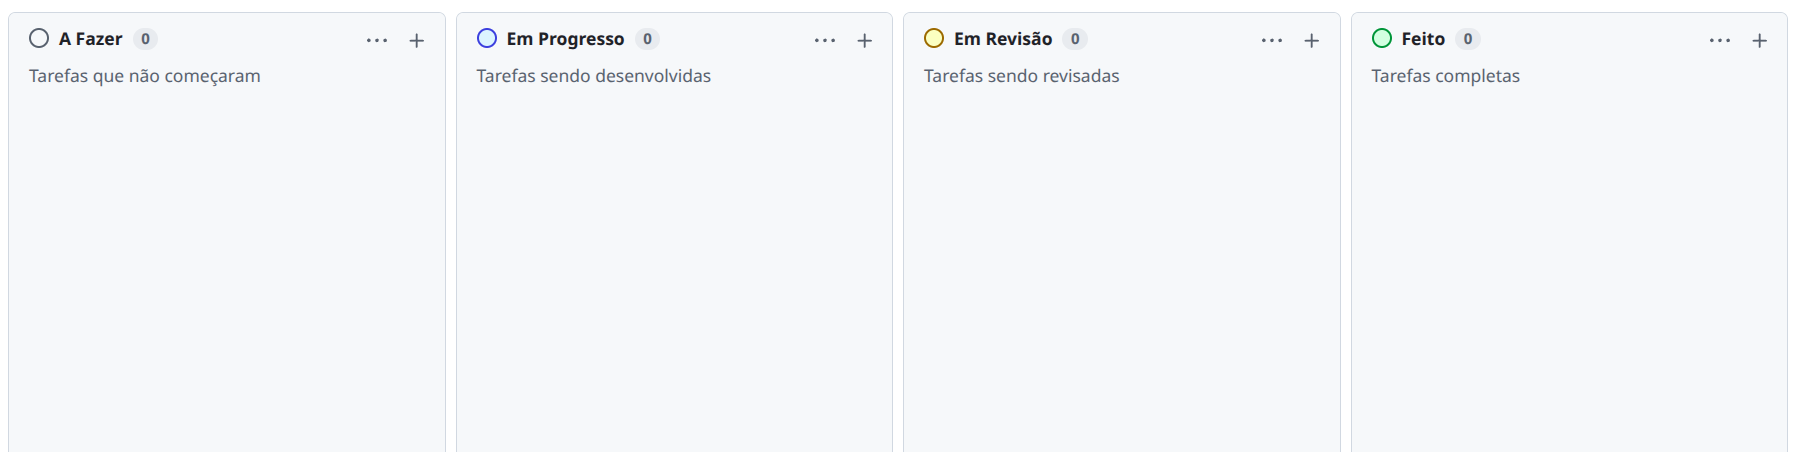
\includegraphics[width=\textwidth]{assets/kanban-github.png}
\vspace{.3cm}
\begin{columns}[T,onlytextwidth]
\column{.60\textwidth}
\textbf{Cada tarefa percorria as etapas do quadro:}\par
A Fazer \(\rightarrow\) Em Progresso \(\rightarrow\) Em Revisão \(\rightarrow\) Feito.
\column{.35\textwidth}
\href{https://github.com/users/EnzoMachad0/projects/1}{\textbf{Abrir o Kanban no GitHub Projects}}
\end{columns}

\note{Tempo: 1.5 minuto(s). Usar a captura exata enviada por Heitor nesta revisão: quatro colunas, sem cartões visíveis, com contadores em zero. A imagem mostra a organização do fluxo e não deve ser usada para contar as tarefas realizadas. Mostrar o quadro pelo link para navegar nos registros disponíveis. Não reutilizar os contadores ou cartões da representação da v0.4. Fonte visual: print fornecido pelo usuário; endereço do GitHub Projects da equipe.}
\end{frame}

\subsection{Branches, revisão e repositório}
% Slide 07 | 1.5 min
\setBGColor{white}
\setLayout{horizontal}
\begin{frame}{Branches e integração por pull request}

\small
\begin{tabularx}{\textwidth}{@{}L{.22\textwidth}Y@{}}
\toprule\head{Etapa} & \head{Exemplo real: correção de inconsistências}\\\midrule
\textbf{Issue} & \href{https://github.com/EnzoMachad0/projeto-dominios/issues/46}{\#46: alinhar os artefatos e a matriz.}\\[.13cm]
\textbf{Branch separada} & \path{docs/consistencia-artefatos}, criada por Danilo.\\[.13cm]
\textbf{Pull request} & \href{https://github.com/EnzoMachad0/projeto-dominios/pull/47}{PR \#47: alterações propostas para a \texttt{main}.}\\[.13cm]
\textbf{Revisão e merge} & Aprovação de Heitor e comentário de revisão de Brenner.\\\bottomrule
\end{tabularx}\par
\vspace{.25cm}\vspace{.3cm}
\textbf{As entregas passavam pela revisão de pelo menos outro integrante antes da integração.}

\note{Tempo: 1.5 minuto(s). Explicar o fluxo de versionamento com um exemplo verificável, sem entrar em comandos Git. Abrir o PR 47 e mostrar as abas Conversation e Files changed. A revisão alinhou códigos de fontes, prioridade de RF07 e RF16 e outros vínculos documentais. A branch de origem é docs/consistencia-artefatos e a base é main. Não afirmar que há proteção automática de branch configurada. Fonte: PR 47 e issue 46 do repositório.}
\end{frame}

% Slide 08 | 1 min
\setBGColor{white}
\setLayout{horizontal}
\begin{frame}{Organização do repositório}

\begin{columns}[T,onlytextwidth]
\column{.52\textwidth}
{\fontsize{9}{12}\selectfont\ttfamily
projeto-dominios/\par
\hspace*{.2cm}README.md\par
\hspace*{.2cm}docs/\par
\hspace*{.5cm}levantamento/\par
\hspace*{.5cm}requisitos/\par
\hspace*{.5cm}casos-de-uso/\par
\hspace*{.5cm}rastreabilidade/\par
\hspace*{.5cm}validacao/\par
\hspace*{.5cm}auditoria/\par
\hspace*{.5cm}entregas/\par}
\column{.43\textwidth}
\kicker{COMO NAVEGAR}
\textbf{README como entrada}\par\vspace{.1cm}Escopo, situação e links.\par
\vspace{.25cm}\textbf{Documentos por finalidade}\par\vspace{.1cm}Fontes, especificação e verificação.\par
\vspace{.25cm}\textbf{Entregas consolidadas}\par\vspace{.1cm}PDF, fontes e apresentação.
\end{columns}
\vspace{.2cm}

\note{Tempo: 1 minuto(s). Abrir o repositório a partir do README e mostrar docs. A árvore é um recorte, não a listagem completa: docs/modelos, dicionario-dados.md e outros arquivos também existem. Distinguir o fonte editável Markdown dos PDFs consolidados. Evitar abrir todas as pastas; mostrar uma cadeia representativa depois. Fonte: árvore local do repositório e README.md.}
\end{frame}

\section{Levantamento de requisitos}
% Slide 09 | 0.4 min
\begingroup\sectionopeningtrue
\setBGColor{white}
\setLayout{horizontal}
\begin{frame}{Levantamento de requisitos}

\begin{columns}[T,onlytextwidth]
\column{.30\textwidth}\num{01}\par\textbf{Entrevista}\par\vspace{.2cm}Necessidades e linguagem\par da professora.
\column{.30\textwidth}\num{02}\par\textbf{Pesquisa geral}\par\vspace{.2cm}Feedback, sistemas,\par privacidade e qualidade.
\column{.30\textwidth}\num{03}\par\textbf{Sistemas análogos}\par\vspace{.2cm}Referências de\par funcionamento e escopo.
\end{columns}
\vspace{.45cm}

\note{Tempo: 0.4 minuto(s). Anunciar as três partes exatamente na ordem solicitada. Explicar a contribuição de cada uma e que observar algo no análogo não equivale à aprovação pelo stakeholder. Os questionários previstos no processo permanecem pendentes. Fonte: docs/PROCESSO\_REQUISITOS.md; docs/requisitos/lista-geral.md.}
\end{frame}
\endgroup

\subsection{Entrevista com a professora}
% Slide 10 | 1.1 min
\setBGColor{white}
\setLayout{horizontal}
\begin{frame}{Entrevista com a professora: o que fizemos}

\begin{columns}[T,onlytextwidth]
\column{.49\textwidth}
\kicker{CONVERSA COM A STAKEHOLDER}
\textbf{Entender o processo}\par
Como a professora caracteriza um feedback e quais situações o sistema deve atender.\par
\vspace{.25cm}
\textbf{Registrar e organizar as respostas}\par
Anotações sobre modalidades, participantes, histórico e acompanhamento.
\column{.46\textwidth}
\kicker{IDEIA CENTRAL DAS ANOTAÇÕES}
{\fontsize{20}{25}\selectfont\bfseries\color{Navy}``comunicar alguém sobre seu desempenho baseado em fatos estabelecidos''\par}
\end{columns}

\note{Tempo: 1.1 minuto(s). Apresentar a professora como stakeholder segundo o contexto informado por Heitor. A frase está nas anotações, não é uma transcrição de gravação: a apresentação corrige apenas acentuação da anotação. O repositório tem E01 e E02, que não devem ser automaticamente atribuídas à mesma pessoa. Fonte: anotações da entrevista, linha 8.}
\end{frame}

% Slide 11 | 1 min
\setBGColor{white}
\setLayout{horizontal}
\begin{frame}{Entrevista: requisitos identificados}

\small
\begin{tabularx}{\textwidth}{@{}L{.44\textwidth}Y@{}}
\toprule\head{Anotação} & \head{Consequência para a especificação}\\\midrule
Documentar fatos e impactos. & Registro contextual de feedback: \textbf{RF21}.\\[.12cm]
Positivo/construtivo; formal/informal. & Duas classificações independentes: \textbf{RF19}.\\[.12cm]
360° e autofeedback. & Modalidades próprias: \textbf{RF17 e RF22}.\\[.12cm]
Plano e pontos de verificação. & Desenvolvimento acompanhado: \textbf{RF18}.\\[.12cm]
Não pode deletar feedback. & Preservação do histórico: \textbf{RN12}.\\\bottomrule
\end{tabularx}\par

\note{Tempo: 1 minuto(s). Relacionar a linguagem original aos identificadores sem ler toda a tabela. Destacar que a especificação está majoritariamente proposta. O plano e a participação do 360° receberam interpretações adicionais, discutidas depois. A existência de RH também está nas notas e aparece nas permissões. Fonte: anotações da entrevista; lista-geral.md; síntese das entrevistas.}
\end{frame}

\subsection{Pesquisa geral}
% Slide 12 | 1.25 min
\setBGColor{white}
\setLayout{horizontal}
\begin{frame}{Pesquisa geral: o que pesquisamos}

\small
\begin{tabularx}{\textwidth}{@{}L{.24\textwidth}YL{.28\textwidth}@{}}
\toprule\head{Eixo da pesquisa} & \head{O que buscamos entender} & \head{Material analisado}\\\midrule
\textbf{Feedback no trabalho} & Fatos e impactos; reconhecimento, melhoria e acompanhamento. & Conceitos sistematizados nas anotações e na síntese.\\[.12cm]
\textbf{Sistemas de feedback} & Ciclos, questionários, múltiplos avaliadores, histórico e resultados. & Enunciado e referências funcionais do levantamento.\\[.12cm]
\textbf{Privacidade dos dados} & Quem acessa as avaliações e como proteger os registros. & LGPD e orientações da ANPD.\\[.12cm]
\textbf{Qualidade do software} & Segurança, clareza de uso e confiabilidade. & ISO/IEC 25010.\\\bottomrule
\end{tabularx}

\note{Tempo: 1.25 minuto(s). Apresentar a pesquisa como entendimento do domínio e das soluções, além das referências legais e de qualidade. Os conceitos de feedback estão sistematizados na síntese das entrevistas (seções 2.1 a 2.5), e os padrões de sistemas aparecem no enunciado e na análise do Culture Amp. A análise aprofundada desse análogo vem na próxima parte. LGPD, ANPD e ISO/IEC 25010 estão documentadas em pesquisa-documental.md. Não atribuir à equipe estudos ou obras específicas que não constam dos arquivos.}
\end{frame}

% Slide 13 | 1 min
\setBGColor{white}
\setLayout{horizontal}
\begin{frame}{Pesquisa geral: requisitos identificados}

\small
\begin{tabularx}{\textwidth}{@{}L{.28\textwidth}YL{.22\textwidth}@{}}
\toprule\head{Conhecimento levantado} & \head{Resposta na especificação} & \head{Registros}\\\midrule
Feedback compreensível & Registrar fatos, impactos e classificação. & \textbf{RF19, RF21}\\[.15cm]
Processo acompanhado & Organizar coletas e consultar histórico e resultados. & \textbf{RF08, RF14--RF16}\\[.15cm]
Transparência sobre os dados & Exibir aviso de privacidade e apoiar acesso aos dados pessoais. & \textbf{RF-DOC-01, 03}\\[.15cm]
Segurança e confiabilidade & Restringir acesso, preservar dados e auditar alterações. & \textbf{RNF01, 06, 07}\\\bottomrule
\end{tabularx}

\note{Tempo: 1 minuto(s). Distinguir requisitos reforçados por fontes complementares de requisitos originados na pesquisa documental. RF19 e RF21 têm origem principal nas entrevistas; RF08 e RF14 a RF16 também estão apoiados no enunciado e nas entrevistas. A pesquisa ajuda a compreender e organizar essas necessidades. RF-DOC-01 e RF-DOC-03 decorrem da pesquisa documental, assim como a consolidação de RNF01, RNF06 e RNF07. Não alterar a origem oficial registrada na lista geral; requisitos documentados permanecem propostas conforme a situação de cada item. Fontes: lista-geral.md, pesquisa-documental.md, síntese das entrevistas e análise do Culture Amp.}
\end{frame}

\subsection{Sistemas análogos}
% Slide 14 | 0.75 min
\setBGColor{white}
\setLayout{horizontal}
\begin{frame}{Sistemas análogos: o que analisamos}

\begin{columns}[c,onlytextwidth]
\column{.49\textwidth}
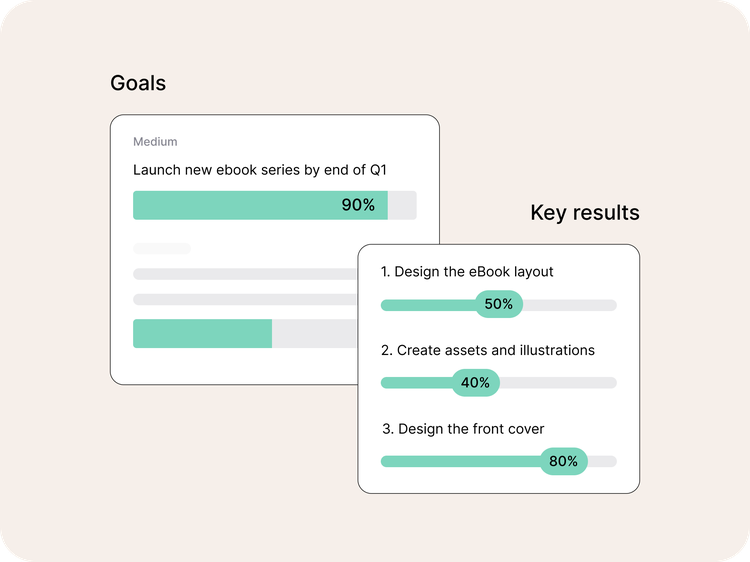
\includegraphics[width=\linewidth,height=4.1cm,keepaspectratio]{assets/cultureamp-metas.png}
\column{.46\textwidth}
\kicker{O RECORTE DA ANÁLISE}
{\large\bfseries Avaliação, feedback\par e desenvolvimento\par}
\vspace{.3cm}
Ciclos e formulários\par\vspace{.18cm}
Múltiplas perspectivas\par\vspace{.18cm}
Metas e acompanhamento
\end{columns}
\vspace{.15cm}

\note{Tempo: 0.75 minuto(s). Descrever o análogo a partir da análise feita pela equipe. A imagem é uma ilustração oficial de acompanhamento de metas, usada para materializar a referência; não é evidência de implementação no projeto. O interesse está nos padrões de processo. Não apresentar a plataforma comercial inteira. Fonte: docs/levantamento/analise-sistema-analogo-culture-amp.md; https://www.cultureamp.com/platform/perform.}
\end{frame}

% Slide 15 | 1 min
\setBGColor{white}
\setLayout{horizontal}
\begin{frame}{Sistemas análogos: requisitos identificados}

\small
\begin{tabularx}{\textwidth}{@{}L{.28\textwidth}YY@{}}
\toprule\head{Aspecto observado} & \head{Aplicação no projeto} & \head{Requisitos / escopo}\\\midrule
Ciclos e questionários & Configuração de coletas. & \textbf{RF08--RF09}\\[.12cm]
Múltiplas fontes & 360° e autoavaliação. & \textbf{RF17, RF22}\\[.12cm]
Desenvolvimento & Plano de ação com progresso. & \textbf{RF18}\\[.12cm]
Calibração e engajamento & Não incorporados ao recorte atual. & Fora do escopo.\\\bottomrule
\end{tabularx}\par
\vspace{.28cm}

\note{Tempo: 1 minuto(s). Escolher um exemplo da tabela e explicar a passagem da observação para a proposta. Não sugerir que recursos comerciais foram copiados integralmente nem confirmados automaticamente. O análogo também apresenta funcionalidades que não fazem sentido para a primeira versão. Fonte: análise do Culture Amp; docs/visao.md, seção 5.}
\end{frame}

\section{Principais requisitos}
% Slide 16 | 0.5 min
\begingroup\sectionopeningtrue
\setBGColor{white}
\setLayout{horizontal}
\begin{frame}{Principais requisitos levantados}

\kicker{DESTAQUES DAS ANOTAÇÕES DA ENTREVISTA}
\begin{columns}[T,onlytextwidth]
\column{.48\textwidth}
\reqitem{01}{Registrar com contexto}{Fatos, impactos e participantes. \textbf{RF21}}
\reqitem{02}{Classificar o feedback}{Formal/informal e positivo/construtivo. \textbf{RF19}}
\column{.48\textwidth}
\reqitem{03}{Ampliar as perspectivas}{Avaliação 360° e autoavaliação. \textbf{RF17, RF22}}
\reqitem{04}{Acompanhar e preservar}{Plano de ação e histórico. \textbf{RF18, RN12}}
\end{columns}

\note{Tempo: 0.5 minuto(s). Os números são contagens da lista geral. Não somar como funcionalidades independentes nem afirmar aprovação dos 36 IDs. Entre os RF principais, RF05 está marcado como validado; os demais estão propostos. Na sequência, destacar as necessidades anotadas na entrevista, não ler o inventário inteiro. Fonte: docs/requisitos/lista-geral.md, seção 3.}
\end{frame}
\endgroup

\subsection{Registro e classificação}
% Slide 17 | 1.25 min
\setBGColor{white}
\setLayout{horizontal}
\begin{frame}{RF21 | Um feedback com contexto}

\small
\begin{tabularx}{\textwidth}{@{}L{.19\textwidth}Y@{}}
\toprule\head{Campo} & \head{Exemplo de registro}\\\midrule
\textbf{Fato} & Na entrega de 12/11, a revisão encontrou três itens sem teste.\\[.1cm]
\textbf{Impacto} & A aprovação precisou de uma nova rodada de revisão.\\[.1cm]
\textbf{Participantes} & Ana (emissora) e Bruno (receptor).\\[.1cm]
\textbf{Classificação} & Formal e construtivo.\\[.1cm]
\textbf{Conteúdo} & Combinar uma verificação de testes antes da próxima entrega.\\\bottomrule
\end{tabularx}\par
\vspace{.22cm}

\note{Tempo: 1.25 minuto(s). Introduzir Ana e Bruno como personagens fictícios para percorrer a apresentação. Mostrar que fato e impacto são diferentes de opinião genérica. O RF21 exige data, participantes, classificação e conteúdo. O questionário pode complementar o registro; não é sinônimo de todo o feedback. A anotação DOCUMENTAR OS FEEDBACKS está representada pelo registro e pelo histórico. Fonte: RF21; RN16; anotações da entrevista, linhas 14 a 21.}
\end{frame}

% Slide 18 | 0.75 min
\setBGColor{white}
\setLayout{horizontal}
\begin{frame}{RF19 | Duas classificações}

\begin{tabularx}{\textwidth}{@{}L{.18\textwidth}YY@{}}
\toprule & \head{Positivo} & \head{Construtivo}\\\midrule
\textbf{Formal} & Reconhecimento em uma avaliação planejada. & Devolutiva estruturada sobre uma melhoria.\\[.3cm]
\textbf{Informal} & Agradecimento após uma colaboração. & Orientação após um evento da rotina.\\\bottomrule
\end{tabularx}\par
\vspace{.35cm}
{\large\bfseries\color{Navy}Formalidade e natureza são independentes.\par}
\vspace{.15cm}

\note{Tempo: 0.75 minuto(s). Explorar as quatro combinações para mostrar que formal não significa construtivo nem informal significa positivo. A classificação fica disponível no histórico. O feedback informal é motivado por um evento e não cria campanha de avaliação. Fonte: RF19 e RF20; anotações da entrevista, linhas 1 e 12.}
\end{frame}

% Slide 19 | 0.75 min
\setBGColor{white}
\setLayout{horizontal}
\begin{frame}{Feedback positivo: reconhecer o efeito}

\begin{columns}[T,onlytextwidth]
\column{.40\textwidth}
\kicker{ESTRUTURA ANOTADA}
\textbf{O que fez de bom}\par\vspace{.25cm}
\textbf{Impactos positivos}\par\vspace{.25cm}
\textbf{Benefícios gerados}\par\vspace{.25cm}
{\color{Muted}Para a chefia, o time\par e a organização.}
\column{.55\textwidth}
{\large\color{Navy}``Você revisou o material\par antes da reunião.\par\vspace{.2cm}
Isso evitou retrabalho\par e permitiu ao time\par concluir a apresentação\par no prazo.''\par}

\end{columns}

\note{Tempo: 0.75 minuto(s). Retomar literalmente o sentido da anotação sobre estrutura positiva: comportamento, bons impactos e benefícios. O exemplo não é um registro real. A síntese SIN-RF07 já contém essa orientação; o RF21 é genérico e ainda precisa detalhar como o sistema apoia o preenchimento. Não declarar esses passos como campos obrigatórios já validados. Fonte: anotações da entrevista, linha 24; SIN-RF07; RF21.}
\end{frame}

% Slide 20 | 1 min
\setBGColor{white}
\setLayout{horizontal}
\begin{frame}{Feedback construtivo: gerar uma ação}

\small
\begin{tabularx}{\textwidth}{@{}L{.28\textwidth}Y@{}}
\toprule\head{Estrutura da entrevista} & \head{Exemplo fictício}\\\midrule
\textbf{Reconhecer} & A revisão do código foi cuidadosa.\\[.1cm]
\textbf{Apresentar fatos} & Três itens chegaram sem testes na última entrega.\\[.1cm]
\textbf{Promover reflexão} & O que podemos fazer para isso não se repetir?\\[.1cm]
\textbf{Combinar uma ação} & Usar um checklist antes de pedir revisão.\\[.1cm]
\textbf{Verificar} & Conferir as próximas quatro entregas.\\\bottomrule
\end{tabularx}\par
\vspace{.2cm}

\note{Tempo: 1 minuto(s). Destacar a sequência anotada pela professora, especialmente a reflexão e a verificação. Explicar a diferença entre apoiar uma boa conversa e exigir mecanicamente elogios em qualquer situação. O sistema não julga a qualidade do feedback automaticamente; registra contexto, ação e evidências. A operacionalização desses passos permanece uma lacuna nos RF oficiais. Fonte: anotações da entrevista, linha 26; SIN-RF08; RF18 e RF21.}
\end{frame}

\subsection{Avaliação e desenvolvimento}
% Slide 21 | 0.75 min
\setBGColor{white}
\setLayout{horizontal}
\begin{frame}{RF17 e RF22 | Perspectivas de avaliação}

\begin{columns}[c,onlytextwidth]
\column{.46\textwidth}
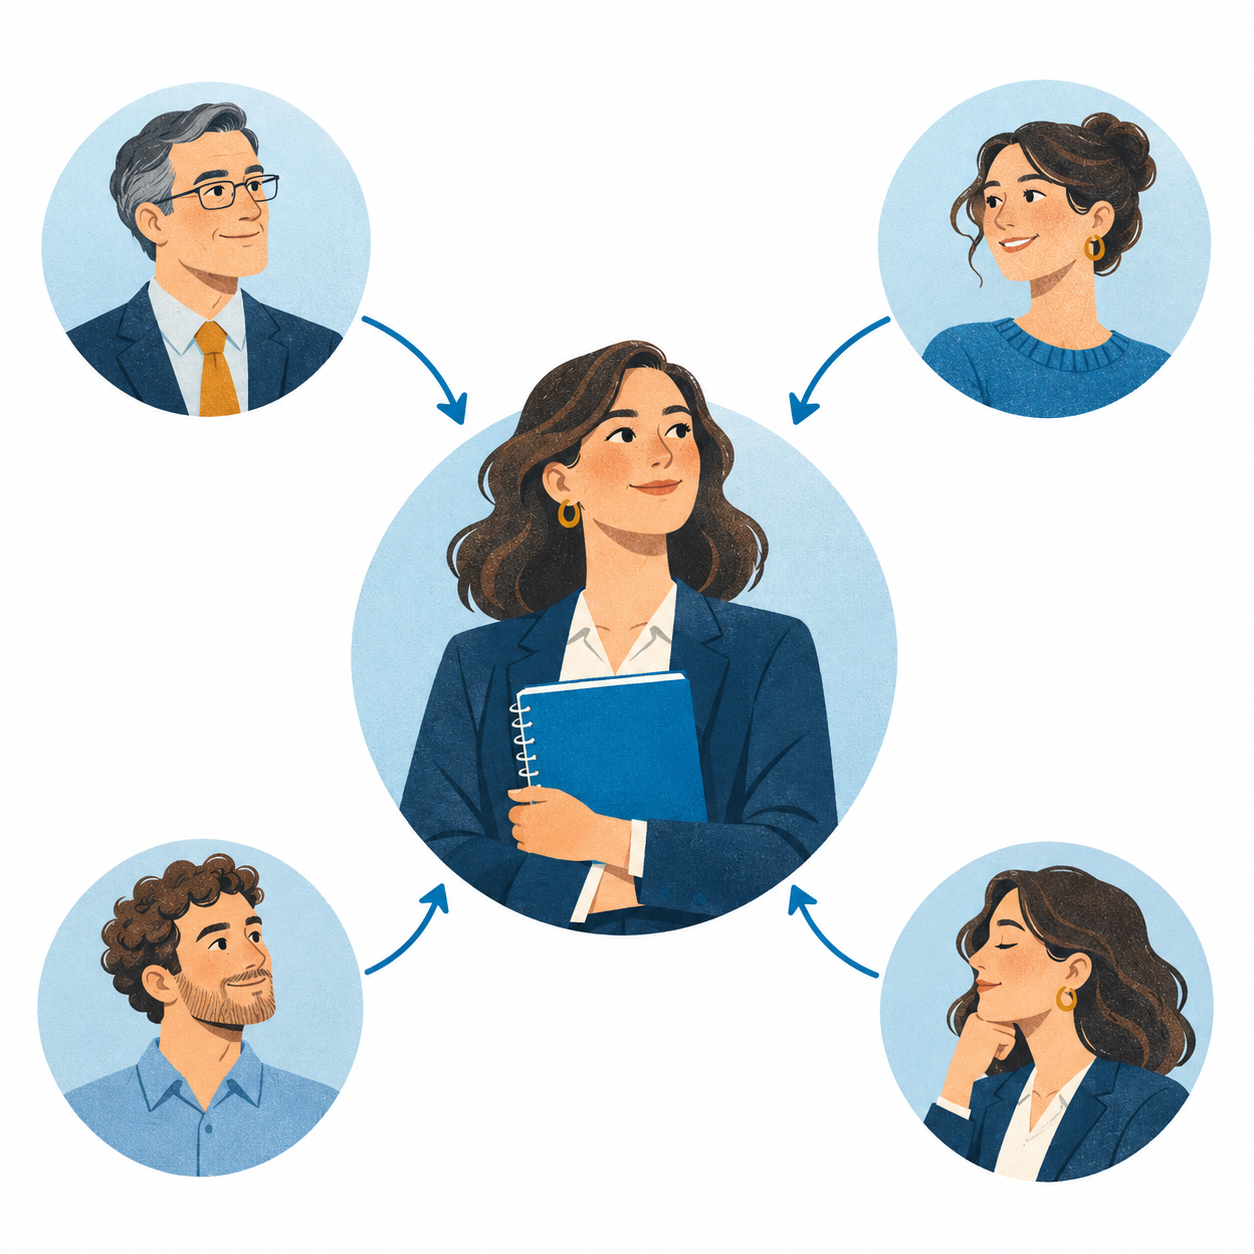
\includegraphics[height=4.3cm]{assets/avaliacao-360.png}
\column{.51\textwidth}
\small
\begin{tabularx}{\linewidth}{@{}lY@{}}
\textbf{Gestor} & Liderança direta.\\[.18cm]
\textbf{Colegas} & Trabalho conjunto.\\[.18cm]
\textbf{Subordinados} & Perspectiva sobre a gestão.\\[.18cm]
\textbf{Próprio avaliado} & Autoavaliação.
\end{tabularx}\par

\end{columns}

\note{Tempo: 0.75 minuto(s). Ilustração conceitual gerada por IA, não um diagrama do sistema. A anotação diz que o gestor abre e todos participam, mas RF17 permite RH ou gestor selecionar participantes. Definir se todos significa time, pessoas vinculadas ao avaliado ou organização inteira. A proposta atual organiza papéis sem exigir reciprocidade; a autoavaliação tem avaliador igual ao receptor. Fonte: RF17, RF22 e RN15; anotações da entrevista, linhas 2 a 6.}
\end{frame}

% Slide 22 | 1.25 min
\setBGColor{white}
\setLayout{horizontal}
\begin{frame}{RF18 | Plano com verificação observável}

\small
\begin{tabularx}{\textwidth}{@{}L{.24\textwidth}Y@{}}
\toprule\head{Elemento} & \head{Exemplo de plano para Bruno}\\\midrule
\textbf{Meta} & Entregar os próximos quatro itens com testes revisados.\\[.1cm]
\textbf{Ação} & Aplicar checklist antes de solicitar revisão.\\[.1cm]
\textbf{Responsável} & Bruno, com acompanhamento de Ana.\\[.1cm]
\textbf{Prazo e check-ins} & Quatro semanas; conferência semanal.\\[.1cm]
\textbf{Evidência proposta} & Checklist e revisão registrada em cada entrega.\\\bottomrule
\end{tabularx}\par
\vspace{.2cm}

\note{Tempo: 1.25 minuto(s). Mostrar o significado dos parâmetros palpáveis anotados: não basta criar uma meta como melhorar. O projeto já prevê ação, responsável, prazo e ponto de verificação. Evidências e critérios testáveis são detalhamento a revisar. A relação temporal do plano com o feedback será apresentada entre as pendências. Fonte: RF18; RN13; anotações da entrevista, linhas 26 e 29.}
\end{frame}

\subsection{Preservação e qualidade}
% Slide 23 | 0.75 min
\setBGColor{white}
\setLayout{horizontal}
\begin{frame}{RN12 | Preservar o que foi registrado}

\begin{columns}[T,onlytextwidth]
\column{.45\textwidth}
{\fontsize{23}{27}\selectfont\bfseries\color{Navy}``não pode\par deletar\par feedback''\par}
\vspace{.25cm}
\column{.50\textwidth}
\kicker{TRADUÇÃO NA ESPECIFICAÇÃO}
\textbf{Preservar o histórico}\par\vspace{.12cm}RN12: sem exclusão física.\par
\vspace{.25cm}\textbf{Preservar o envio}\par\vspace{.12cm}RF12: respostas imutáveis.\par
\vspace{.25cm}\textbf{Registrar operações}\par\vspace{.12cm}RF16: trilha de auditoria.
\end{columns}

\note{Tempo: 0.75 minuto(s). Explicar que a especificação ampliou a anotação, proibindo exclusão física de todos os dados. Distinguir cancelamento de exclusão e mencionar que a retenção deve ser compatibilizada com as necessidades de proteção de dados. Não declarar o conflito resolvido. Fonte: anotações da entrevista, linha 31; RN12; RF12 e RF16.}
\end{frame}

% Slide 24 | 1 min
\setBGColor{white}
\setLayout{horizontal}
\begin{frame}{Qualidade: como o sistema deve funcionar}

\small
\begin{tabularx}{\textwidth}{@{}L{.20\textwidth}YY@{}}
\toprule\head{Aspecto} & \head{Comportamento esperado} & \head{Referência}\\\midrule
\textbf{Segurança} & Bloquear acesso fora do escopo. & RNF01, RNF07.\\[.18cm]
\textbf{Integridade} & Não duplicar envios nem perder parte das respostas. & RNF02.\\[.18cm]
\textbf{Interação} & Permitir teclado, retomar rascunho e confirmar envio. & RNF03, RNF13.\\[.18cm]
\textbf{Recuperação} & Recuperar os dados após uma falha. & RNF05; metas a validar.\\\bottomrule
\end{tabularx}\par

\note{Tempo: 1 minuto(s). Diferenciar qualidade de funcionalidade. São requisitos propostos, não resultados de ensaios. Evitar citar desempenho como capacidade já comprovada. Conectar cada aspecto a um risco compreensível do processo de avaliação. Fonte: docs/requisitos/especificacao-suplementar.md.}
\end{frame}

\section{Resultados e demonstrações}
% Slide 25 | 0.5 min
\begingroup\sectionopeningtrue
\setBGColor{white}
\setLayout{horizontal}
\begin{frame}{Resultados e demonstrações}
\begin{columns}[T,onlytextwidth]
\column{.46\textwidth}\num{01}\par\textbf{Principais documentos}\par\vspace{.25cm}Papel de cada artefato, exemplos no projeto e vínculos entre requisitos, casos de uso e aceitação.
\column{.46\textwidth}\num{02}\par\textbf{Protótipo no Figma}\par\vspace{.25cm}Percursos de avaliação e acompanhamento nas telas produzidas.
\end{columns}
\note{Tempo: 0.5 minuto(s). Apresentar as duas partes desta seção: principais documentos produzidos e demonstração do Figma. Não há mais um bloco separado de funcionamento esperado.}
\end{frame}
\endgroup

\subsection{Documentos e rastreabilidade}
% Slide 26 | 1.5 min
\setBGColor{white}
\setLayout{horizontal}
\begin{frame}{Os documentos produzidos}
\fontsize{9}{10.5}\selectfont\renewcommand{\arraystretch}{1.0}
\begin{tabularx}{\textwidth}{@{}L{.19\textwidth}YL{.40\textwidth}@{}}
\toprule\head{Documento} & \head{Papel principal} & \head{Exemplo no projeto}\\\midrule
\textbf{Visão} & Delimitar problema, público e escopo. & Perfis RH, gestor e profissional.\\[0cm]
\textbf{Requisitos} & Especificar comportamentos, regras e qualidade. & RF21: contexto do feedback; RF12: envio imutável.\\[0cm]
\textbf{Casos de uso} & Descrever interações, alternativas e garantias. & CU-02: responder, salvar rascunho e confirmar envio.\\[0cm]
\textbf{Dicionário} & Padronizar termos, dados e restrições. & Avaliação, coleta e resposta; tipos de nota e Sim/Não.\\[0cm]
\textbf{Rastreabilidade} & Conectar origem, requisito e verificação. & RF12 $\rightarrow$ CU-02 $\rightarrow$ CA08.\\[0cm]
\textbf{Documentação mestre} & Consolidar e orientar a leitura dos artefatos. & Síntese da etapa e referências aos documentos completos.\\\bottomrule
\end{tabularx}
\vspace{.2cm}\href{https://github.com/EnzoMachad0/projeto-dominios/tree/main/docs}{\textbf{Abrir os documentos no repositório}}
\note{Tempo: 1.5 minuto(s). Apresentar o papel de cada documento e a pergunta que ele responde. Visão: por que o sistema existe e para quem? Requisitos: o que precisa fazer e respeitar? Caso de uso: como a interação acontece, inclusive nas falhas? Dicionário: qual o significado dos dados? Rastreabilidade: de onde veio e como conferir? Documentação mestre: onde encontrar a síntese da etapa? Exemplos são extraídos de docs/visao.md, requisitos, CU-02, dicionario-dados.md e matriz-rastreabilidade.md. A seguir, aprofundar três documentos e demonstrar seus arquivos.}
\end{frame}

% Slide 27 | 2 min
\setBGColor{white}
\setLayout{horizontal}
\begin{frame}{Especificação de requisitos}
\begin{columns}[c,onlytextwidth]
\column{.48\textwidth}
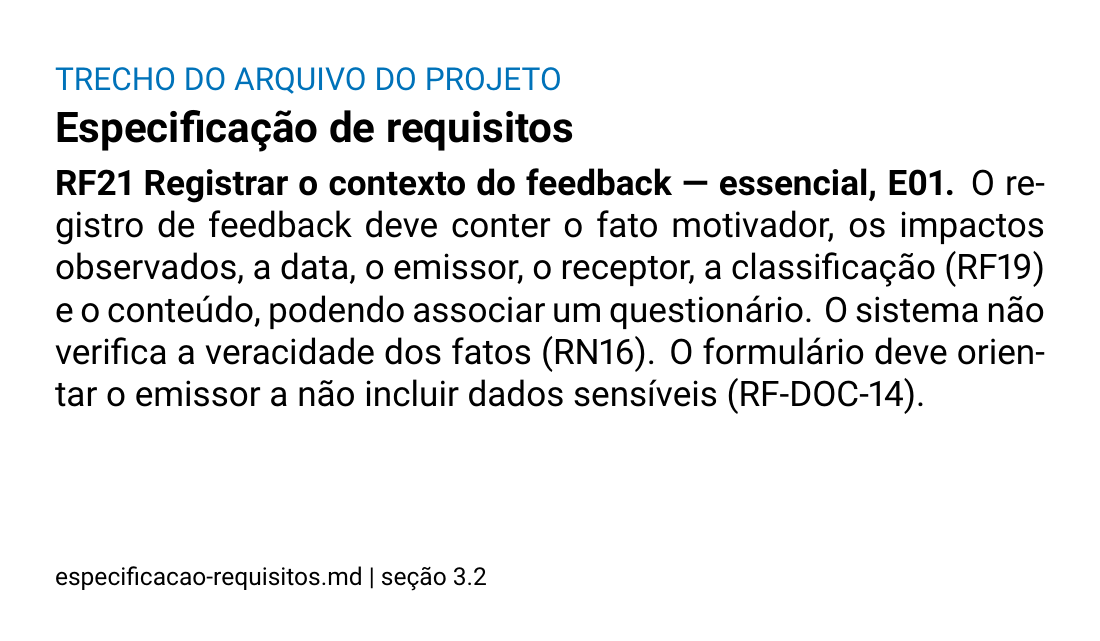
\includegraphics[width=\linewidth,height=4.1cm,keepaspectratio]{assets/trecho-requisitos.png}
\column{.48\textwidth}
\small
\kicker{PAPEL PRINCIPAL}
Definir comportamentos, regras e critérios de aceitação do sistema.\par
\vspace{.12cm}\textbf{Exemplos no projeto}\par
\textbf{RF21}: registrar fato, impacto, participantes e classificação.\par\vspace{.12cm}
\textbf{RF12 e CA08}: confirmar um único envio e impedir alterações posteriores.\par
\vspace{.12cm}\textbf{Como usamos}: referência para detalhar casos de uso, telas e critérios de aceitação.
\end{columns}
\vspace{.18cm}\href{https://github.com/EnzoMachad0/projeto-dominios/blob/main/docs/requisitos/especificacao-requisitos.md}{\textbf{Abrir a especificação completa}}
\note{Tempo: 2 minuto(s). Abrir a especificação e mostrar sua organização: funcionalidades, regras de negócio, requisitos de qualidade e critérios de aceitação. Ler o trecho RF21 como exemplo de requisito com contexto do feedback. Depois localizar RF12 e CA08 para mostrar que a descrição do comportamento tem uma forma concreta de verificação: avaliação completa, envio único, respostas imutáveis e avaliação inversa independente. Na lista geral, mostrar fonte, prioridade e situação. O papel do documento é orientar uma implementação verificável; não afirmar que os testes ou a implementação já foram executados.}
\end{frame}

% Slide 28 | 2 min
\setBGColor{white}
\setLayout{horizontal}
\begin{frame}{Caso de uso completo}
\begin{columns}[c,onlytextwidth]
\column{.48\textwidth}
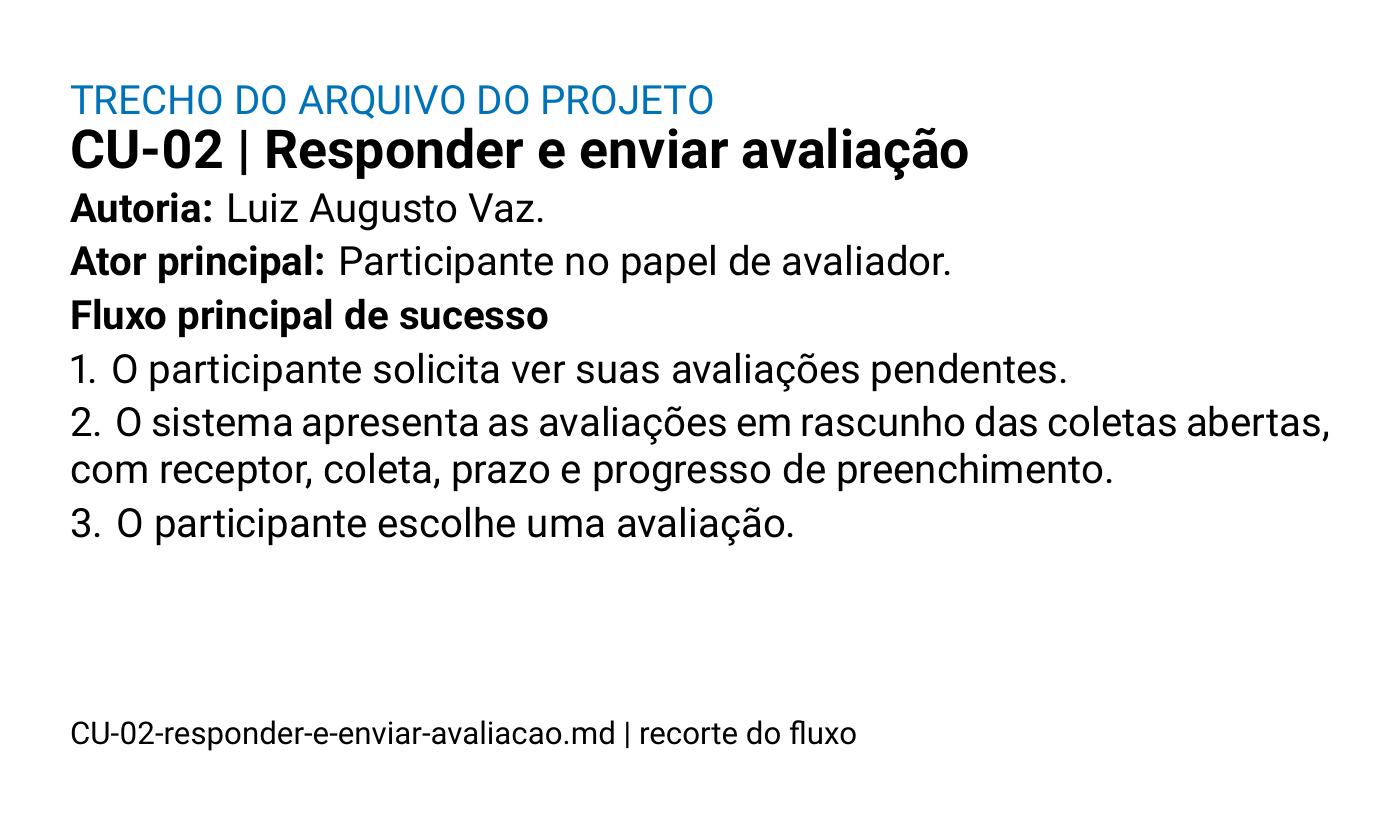
\includegraphics[width=\linewidth,height=4.1cm,keepaspectratio]{assets/trecho-caso-de-uso.png}
\column{.48\textwidth}
\small
\kicker{PAPEL PRINCIPAL}
Detalhar a interação entre participante e sistema para atingir um objetivo, incluindo alternativas e falhas.\par
\vspace{.12cm}\textbf{CU-02: responder e enviar avaliação}\par
Selecionar pendência $\rightarrow$ responder $\rightarrow$ salvar rascunho $\rightarrow$ revisar e confirmar envio.\par
\vspace{.12cm}\textbf{Exemplos de exceção}\par
Nota 6 em escala de 0 a 5: rejeitar o valor.\par
Pergunta sem resposta: impedir o envio.\par
Falha no envio: preservar o rascunho.
\end{columns}
\vspace{.18cm}\href{https://github.com/EnzoMachad0/projeto-dominios/blob/main/docs/casos-de-uso/CU-02-responder-e-enviar-avaliacao.md}{\textbf{Abrir o CU-02 completo}}
\note{Tempo: 2 minuto(s). Demonstrar o CU-02, de autoria de Luiz Augusto Vaz. O ator é o participante no papel de avaliador, que pode ter perfil RH, Gestor ou Profissional. Pré-condições: autenticação, coleta aberta dentro do período e avaliação atribuída em rascunho. Mostrar o fluxo até a confirmação do envio e as garantias de sucesso: ENVIADA, respostas válidas e imutáveis, envio único e independência da avaliação inversa. Abrir a extensão 6a (valor inválido), 8a (perguntas pendentes) e 11c (falha com reversão integral). Relacionar RF11/RF12 e CA07/CA08. Fonte: docs/casos-de-uso/CU-02-responder-e-enviar-avaliacao.md.}
\end{frame}

% Slide 29 | 2 min
\setBGColor{white}
\setLayout{horizontal}
\begin{frame}{Matriz de rastreabilidade}
\begin{columns}[c,onlytextwidth]
\column{.48\textwidth}
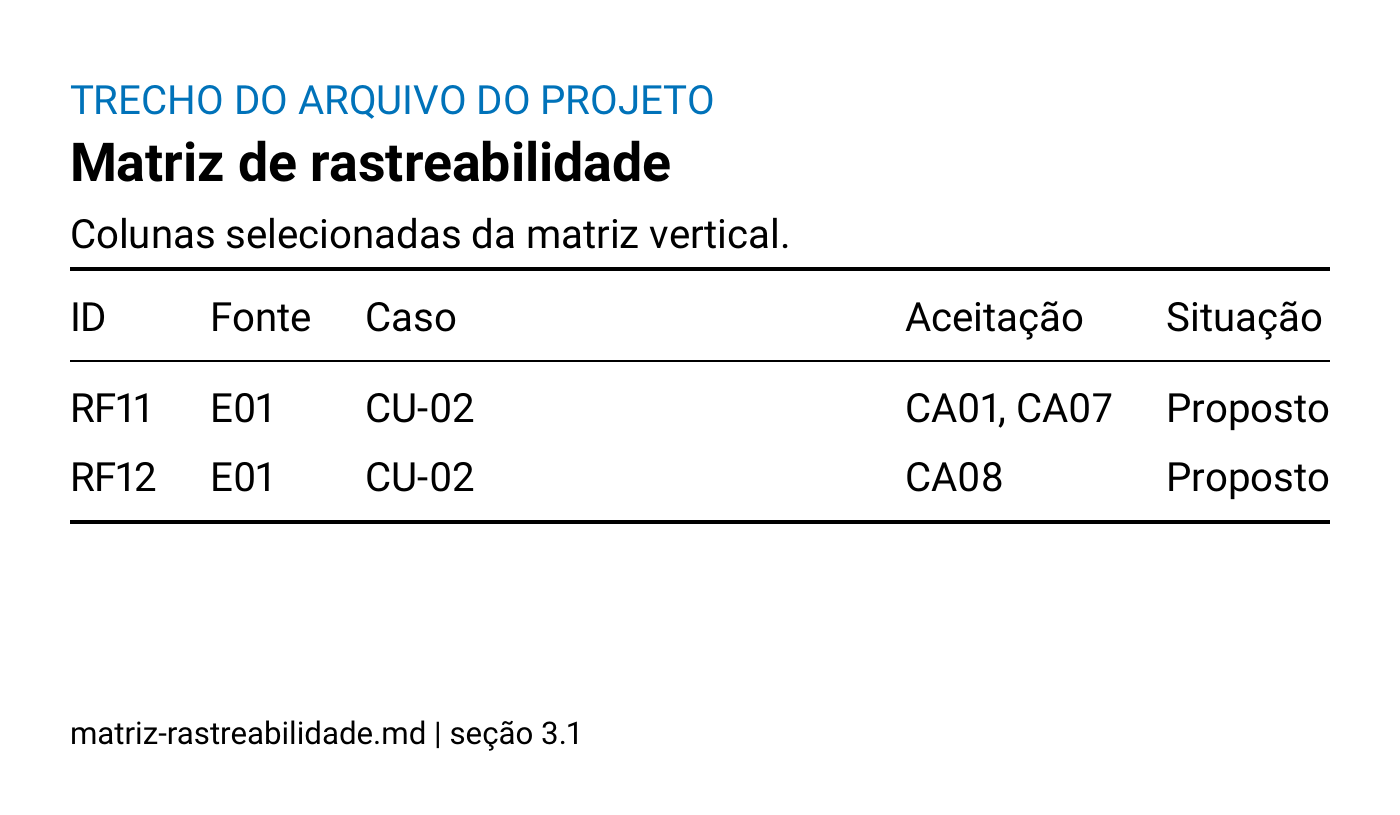
\includegraphics[width=\linewidth,height=4.1cm,keepaspectratio]{assets/trecho-rastreabilidade.png}
\column{.48\textwidth}
\small
\kicker{PAPEL PRINCIPAL}
Conectar a fonte da necessidade ao requisito, ao caso de uso e à verificação.\par
\vspace{.12cm}\textbf{Exemplo no projeto}\par
Entrevista E01 $\rightarrow$ \textbf{RF12} (enviar avaliação) $\rightarrow$ \textbf{CU-02} $\rightarrow$ \textbf{CA08}.\par
\vspace{.12cm}\textbf{Como usamos}\par
Conferir cobertura, localizar lacunas e identificar os documentos afetados por uma mudança.
\end{columns}
\vspace{.18cm}\href{https://github.com/EnzoMachad0/projeto-dominios/blob/main/docs/rastreabilidade/matriz-rastreabilidade.md}{\textbf{Abrir a matriz completa}}
\note{Tempo: 2 minuto(s). Abrir as linhas RF11 e RF12 da matriz. RF11 se liga a E01, CU-02 e CA01/CA07; RF12 se liga a E01, CU-02 e CA08. Percorrer o vínculo nos dois sentidos: a fonte justifica a necessidade, o caso de uso detalha a interação e o critério de aceitação define o que conferir. Exemplificar impacto: uma mudança no envio exige conferir RF12, CU-02 e CA08. A matriz também mantém situação e relações com outros artefatos, embora esta apresentação não detalhe a modelagem. As figuras mostram colunas selecionadas do documento real.}
\end{frame}

% Slide 30 | 1.5 min
\setBGColor{white}
\setLayout{horizontal}
\begin{frame}{Demonstração: seguir uma informação}

\begin{tabularx}{\textwidth}{@{}L{.10\textwidth}L{.27\textwidth}Y@{}}
\toprule & \head{Abrir} & \head{O que mostrar}\\\midrule
\head{01} & \href{https://github.com/EnzoMachad0/projeto-dominios}{\textbf{README}} & Situação do projeto e links dos artefatos.\\[.15cm]
\head{02} & \href{https://github.com/EnzoMachad0/projeto-dominios/blob/main/docs/requisitos/lista-geral.md}{\textbf{Lista geral}} & Fonte, prioridade e situação do RF12.\\[.15cm]
\head{03} & \href{https://github.com/EnzoMachad0/projeto-dominios/blob/main/docs/casos-de-uso/CU-02-responder-e-enviar-avaliacao.md}{\textbf{CU-02}} & Detalhamento da resposta e envio da avaliação.\\[.15cm]
\head{04} & \href{https://github.com/EnzoMachad0/projeto-dominios/blob/main/docs/rastreabilidade/matriz-rastreabilidade.md}{\textbf{Matriz}} & Vínculo com a verificação CA08.\\\bottomrule
\end{tabularx}\par
\vspace{.25cm}

\note{Tempo: 1.5 minuto(s). Navegar nos arquivos seguindo uma informação real: README para localizar a documentação; lista geral para fonte, prioridade e situação do RF12; CU-02 para resposta em rascunho e envio; matriz para o vínculo com CA08. Abrir o critério CA08 na especificação e conferir as garantias: único envio e imutabilidade. Usar os arquivos locais selecionados no pacote se a rede falhar. Reservar o tempo para mostrar os arquivos, sem ler apenas a tabela.}
\end{frame}

\subsection{Protótipo e percursos}
% Slide 31 | 0.5 min
\setBGColor{white}
\setLayout{horizontal}
\begin{frame}{Protótipo PulsarRH}

\begin{columns}[c,onlytextwidth]
\column{.40\textwidth}
\centering\qrcode[height=3.45cm]{https://www.figma.com/design/pD7rcKYlK7cQ0M5KidV1kL/PulsarRH?node-id=1-3}
\column{.55\textwidth}
\kicker{DEMONSTRAÇÃO NO FIGMA}
{\large\bfseries Ver o percurso,\par discutir as decisões\par de interface\par}
\vspace{.4cm}
\href{https://www.figma.com/design/pD7rcKYlK7cQ0M5KidV1kL/PulsarRH?node-id=1-3}{\textbf{Abrir o arquivo PulsarRH}}
\vspace{.25cm}\par
\end{columns}

\note{Tempo: 0.5 minuto(s). Abrir previamente o Figma e usar o link clicável ou QR. O conector não permitiu acesso ao arquivo durante a preparação desta versão; não foram inventadas capturas. O percurso a seguir deve ser adaptado ao que realmente estiver representado. Não apresentar imagens conceituais desta apresentação como telas do Figma. Fonte: README.md; link do protótipo; matriz de rastreabilidade, L03.}
\end{frame}

% Slide 32 | 1.75 min
\setBGColor{white}
\setLayout{horizontal}
\begin{frame}{Percurso 1 | Organizar uma avaliação}

\small
\begin{tabularx}{\textwidth}{@{}L{.24\textwidth}YY@{}}
\toprule\head{No protótipo} & \head{O que observar} & \head{Requisito}\\\midrule
\textbf{Perfil e acesso} & É claro qual é o escopo do usuário? & RF01.\\[.2cm]
\textbf{Configuração} & Período e questionário estão compreensíveis? & RF08.\\[.2cm]
\textbf{Participantes} & Quem avalia quem fica explícito? & RF09, RF17.\\[.2cm]
\textbf{Confirmação} & O efeito da abertura está claro? & RF09.\\\bottomrule
\end{tabularx}\par
\vspace{.25cm}

\note{Tempo: 1.75 minuto(s). Reservar o tempo para navegar no Figma, em vez de ler o slide. Posicionar o protótipo no perfil administrativo, se essa área existir. Relacionar o que está na interface às decisões de período, questionário e participantes. Não simular funcionalidades indisponíveis. Explicar eventuais lacunas usando a tabela como critério de observação. Se o acesso ao Figma falhar durante a apresentação, usar o tempo para discutir as decisões esperadas, sem alegar demonstração concluída. Fonte: RF01, RF08, RF09, RF17; matriz de rastreabilidade, L03.}
\end{frame}

% Slide 33 | 1.75 min
\setBGColor{white}
\setLayout{horizontal}
\begin{frame}{Percurso 2 | Responder e acompanhar}

\small
\begin{tabularx}{\textwidth}{@{}L{.24\textwidth}YY@{}}
\toprule\head{No protótipo} & \head{O que observar} & \head{Requisito}\\\midrule
\textbf{Resposta} & Campos e tipo de resposta claros. & RF11.\\[.2cm]
\textbf{Envio} & Consequência e confirmação explícitas. & RF12.\\[.2cm]
\textbf{Histórico} & Contexto e classificação recuperáveis. & RF14, RF21.\\[.2cm]
\textbf{Plano} & Meta e verificação compreensíveis. & RF18.\\\bottomrule
\end{tabularx}\par
\vspace{.25cm}

\note{Tempo: 1.75 minuto(s). Demonstrar apenas as telas existentes. Procurar clareza sobre quem verá a resposta, possibilidade de retomar e confirmação do envio. Relacionar o registro de fatos à devolutiva e ao desenvolvimento. O protótipo não valida persistência nem cálculo dos indicadores. A matriz ainda não liga cada tela aos requisitos; essa é uma pendência de rastreabilidade. Fonte: RF11, RF12, RF14, RF18 e RF21; matriz de rastreabilidade, L03.}
\end{frame}

\section{Encerramento}
\subsection{Síntese das entregas}
% Slide 34 | 1 min
\begingroup\sectionopeningtrue
\setBGColor{white}
\setLayout{horizontal}
\begin{frame}{Encerramento}
\kicker{SÍNTESE DAS ENTREGAS}
\begin{columns}[T,onlytextwidth]
\column{.54\textwidth}
{\fontsize{23}{28}\selectfont\bfseries\color{Navy}Feedback com contexto.\par\vspace{.15cm}Desenvolvimento com acompanhamento.\par}
\column{.41\textwidth}
\textbf{O que o trabalho produziu}\par\vspace{.2cm}
Necessidades levantadas\par\vspace{.12cm}
Requisitos documentados\par\vspace{.12cm}
Casos de uso e critérios de aceitação\par\vspace{.12cm}
Protótipo e arquivos organizados
\end{columns}
\note{Tempo: 1 minuto(s). Encerrar com as contribuições efetivamente produzidas. O principal resultado é a explicitação das necessidades e das decisões, não uma aplicação em produção. Relembrar que o acompanhamento é central para avaliar o efeito do feedback. Agradecer e abrir o tempo de reserva para perguntas. A equipe completa consta no preâmbulo e neste roteiro. Fonte: README.md; documento de visão; pauta de validação.}
\end{frame}
\endgroup

\end{document}
